


\chapter{Bootstrap}
 


\section {Introduction}


Applying deep learning to new domains usually implies a considerable data collection problem. We look at idea of how we can use a partially trained model as an aid to a human annotator. We do this by providing the partially trained model's prediction as a starting point for a human annotator to directly edit. This is demonstrated by applying our ideas to building a small segmentation dataset for labeling trees in a plantation. We also show that by starting with a pre--trained model and fine--tuning, we can provide a useful aid to a human annotator using very few input images.


One of the greatest problems faced in machine learning is obtaining accurate and sufficient annotated data where typically thousands of examples are required. Deep learning has been shown to perform well on large datasets, and there exists a variety of large datasets in the public domain for research purposes. Applying deep learning to a new application presents a data collection and annotation problem, for which there are a number of active research topics such as active learning, semi-supervised learning, and interactive machine learning. We discuss these topics in more detail below.

Not only is it necessary to collect and annotate data - one of the primary questions asked when considering the use of machine learning is 'How many examples are necessary?'. To which the usual answer is to by experimental validation where part of the data is held back and used to test the effectiveness of training on the other part.

We present a bootstrapping method for creating a segmentation dataset guided by a feedback loop using a human annotator and a model (a \gls{CNN}). We use segmentation as our task because it is applicable to many domains and is very flexible, for example, labelling tree branches using axis aligned bounding boxes is in-feasible. Our approach is based on using a partially trained model to assist the human annotator.

We show that by using transfer learning by fine tuning a pre--trained model, very few hand annotated images are necessary to provide a good level of assistance to a human annotator, using the related idea that recognition is better than recall. Just as it is much faster to recognise a solution rather than recall one from memory, if a model can produce an annotation which is mostly correct - a human can recognise and fix small problems much faster than reproducing the annotation from scratch. At worst the human annotator can discard the automatic solution and produce the annotation by hand, and learn a measure of the model's current level.

\begin{figure}[h]
\centering
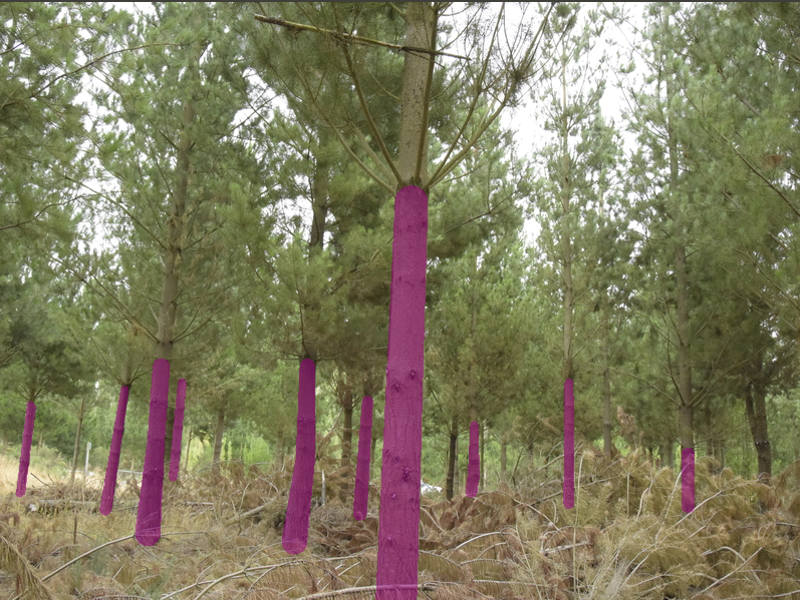
\includegraphics[width=0.9\linewidth]{bootstrap/trees_example.png}

\caption{Example from the trees dataset}
\label{fig:tree}
\end{figure}

\subsection{Related methods}


Human time becomes the main expense when annotating data, so in order to minimise cost there exist strategies such as crowd sourcing. In order to get a lot of people to contribute there exist methods such as gamification, e.g. a game Quick Draw \cite{Ha2017}, or presenting the task as proof of human--ness \cite{Goodfellow2013a}.  Most annotations performed on a large scale rely on brute labour, with many using global markets such as \gls{AMT}. Large scale datasets such as ImageNet \cite{Russakovsky2015} are built with \gls{AMT}. 

The closest related work to ours we have found, with a very similar idea is \cite{Papadopoulos2016}. Instead of annotating a dataset from scratch - they iteratively improve a partially trained model by asking questions of a human annotator. They initially bootstrap a model using semi-supervised methods with per--image labels. A simple Yes/No questioning process is then used used to annotate a dataset by refining bounding boxes proposed by the model (and intelligently prune bounding box proposals by adjusting thresholds and overlap \gls{IOU}). They report the speedup to achieve nearly equivalent accuracy of $6\times$ to $9\times$.

A closely related research area is active learning. The motto of active learning is ``putting the model in the loop'' (or conversely the human, depending on the perspective). Active learning requires a model with some estimate of uncertainty. Given a pool of non annotated examples, an algorithm can choose which examples require human annotation (because the model is uncertain), or go with the model's annotation (because the model is certain). One recent example, using active learning for segmentation is \cite{Xu2017}, where they focus on finding the nodes (super pixels) which induce the largest change in a \gls{CRF} model .

Semi-supervised machine learning attempts to use existing knowledge or domain properties to infer annotations. For example using motion cues to give indications of object boundaries \cite{Hong2017}, or using an image classifier to perform object detection by blanking out portions of the image, so as to determine which parts are important \cite{Bazzani2016}. Semi-supervised methods often substitute for human labour, but in doing so make sacrifices of the quality and often result in somewhat noisy data. As a result semi-supervised methods are often used as a means of bootstrapping a model before involving a human annotator, for example as used in \cite{Papadopoulos2016}.


\subsection {Assisted annotation}


\begin{figure}[h]
\centering
\begin{subfigure}{.25\textwidth}
  \centering
  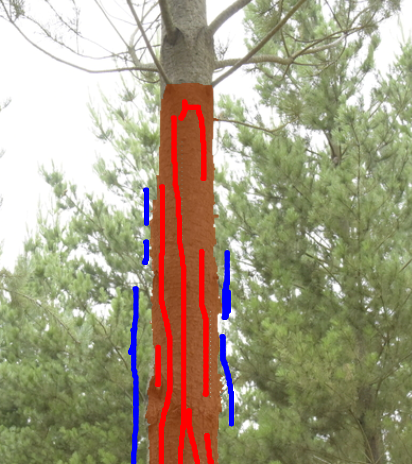
\includegraphics[width=0.5\linewidth]{bootstrap/labelme.png}
  \caption{Labelme mask annotation}  
  \label{fig:labelme}
\end{subfigure}%
\begin{subfigure}{.25\textwidth}
  \centering
  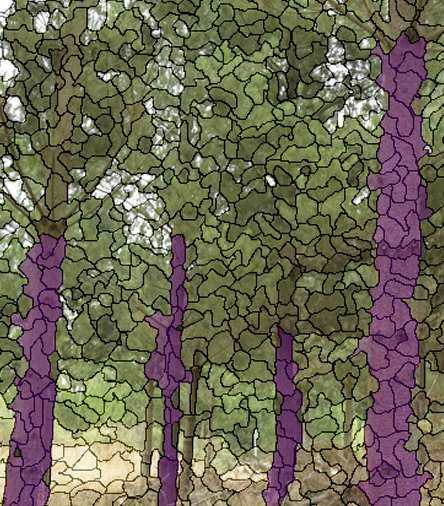
\includegraphics[width=.5\linewidth]{bootstrap/superpixels.png}
  \caption{Annotation using super pixels}
  \label{fig:superpixels}
\end{subfigure}

\caption{Assisted annotation methods}
\label{fig:annot_method}
\end{figure}


In our initial attempts to annotate a dataset, one of the problems was often that using the assisted annotation tools such as the mask tool in the LabelMe \cite{Russell2007} interface actually required more work than manually annotating the polygon boundary from scratch. The LabelMe mask tool provides a GrabCut--esque interface where positive and negative stripes can be painted onto an image. Our experience in creating a mask for a tree trunk can be seen in Figure \ref{fig:labelme} where annotations are bright red and green. The initial painted stripe provided a rough outline, but many small annotations were needed to make the mask resemble the true edge of the tree trunk.

In \cite{Galloway2017}, the images are segmented using superpixels (clusters of pixels grouped with an unsupervised algorithm), where labelling groups of pixels is substantially less work than labelling individual pixels, and superpixels seem to do well at finding image boundaries where \gls{CNN} are often imprecise. This does present some difficulties, such as the ambiguity where multiple classes are covered in one superpixel. In our experiences using superpixels provided imprecise boundaries and saved little time, an example of our tool with superpixel selection is shown in Figure \ref{fig:superpixels}.

Deep learning has previously been used to aid in object instance selection. In \cite{Xu2016} a \gls{FCN} is trained to perform semantic segmentation of objects in images as selected by users. Users click on an object (providing positive and negative points), which are passed to the model as distance maps along with the regular colour image data. Another recent approach is that of \cite{Xu2017} which also aims at interactive instance segmentation, using a rectangle as an input (also using a distance map), and producing an instance segmentation.

% \begin{figure*}[!ht]
% \centering

% \end{figure*}




\section{Proposed Method}

Our approach is to annotate data and train a model as we go. First annotate a small number of examples to begin with to create an initial training set, and use these examples to train an initial model. New examples are then classified by the model, at which point the human annotator fixes any mistakes and the corrected example is added to the training set. Initially the annotator will need to fix the majority of the data, and as the model improves such feedback will be required less and less. The idea is that the model will quickly learn the easy cases, which can be quickly ignored to save work, and the annotator will be left to invervene only with the more important challenging cases.

We have used this method to build a small scale tree trunk segmentation dataset, a prototype for the purposes of an automated drone tree pruning project for the purpose of pruning lower branches off young Pinus Radiata tree plantations. Our work is intended to allow the drone see the trees despite the forest. To evaluate methods of dataset construction and evaluate methods of annotation, we wrote an annotation application written with a Qt interface, with tools for drawing on masks and iterating the dataset and refining model proposed annotations.

Our workflow after first training some initial number of examples was to leave a training process in the background which would pick up newly created annotations after each training epoch. 


\subsection {Models}

\begin{figure}[h]
  \centering
  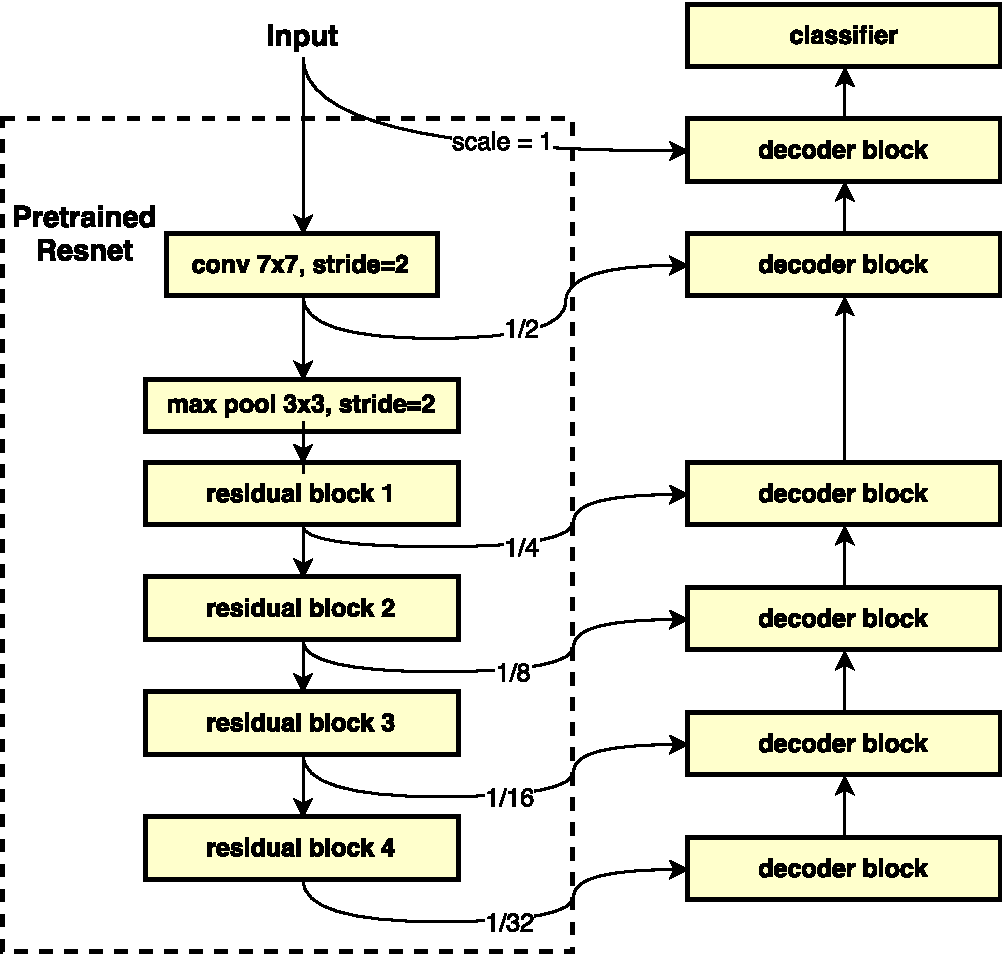
\includegraphics[width=0.9\linewidth]{bootstrap/network.pdf}
  \caption{Encoder--decoder network with pre-trained Resnet}  
  \label{fig:network}
\end{figure}
\begin{figure}
  \centering
  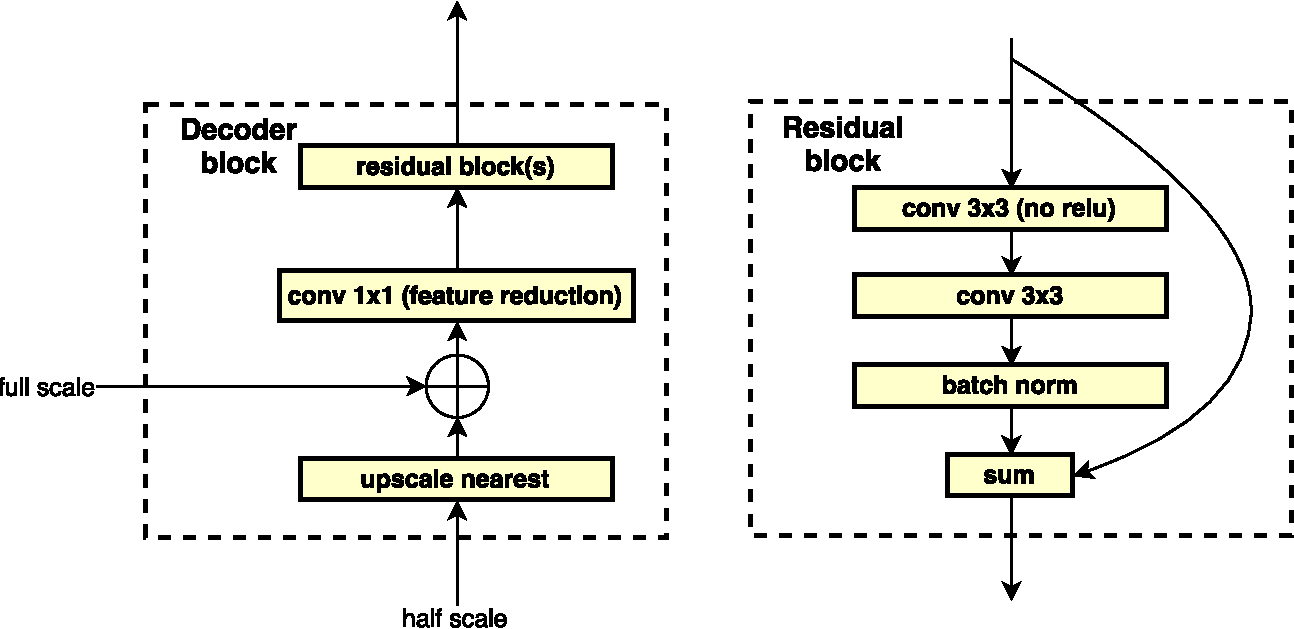
\includegraphics[width=0.9\linewidth]{bootstrap/network_blocks.pdf}
  \caption{Block sub networks}  
  \label{fig:decode_block}
\end{figure}

For our image segmentation model we have used an encoder--decoder with skip connections similar to UNet \cite{Ronneberger2015} (utilizing padding and without cropping the skip connections). Each level of the encoder and decoder (at the same resolution) are connected by a skip connection bypassing the lower layers of the network. We focus on two architectures, the first is a pre-trained ResNet model as an encoder with a decoder added, and the second is a symmetrical encoder and decoder. We refer to the first as ``pre-trained and the second as ``ladder'' in the experiments below.

The architecture based on the pre-trained ResNet is shown in Figure \ref{fig:network}, with the decoder and residual block used shown in Figure \ref{fig:decode_block}. The particular ResNet we use is the ``resnet18'' from the Pytorch model zoo, (the smallest of the various ResNet architectures) with weights trained on the ImageNet dataset. 

Our decoder for the ``pre-trained model uses a single residual block at the point labelled ``residual block(s)'' in Figure \ref{fig:decode_block}. The ``ladder'' model uses residual blocks of size (1, 2, 3, 3, 3, 3) in both encoder and decoder. Our decoder uses $ 1x1 $ convolutions to reduce the feature sizes coming from intermediate layers of the ResNet, the number of features used in the decoder is 16, with 8 additional features at each layer further down. An implicit Batch Normalisation layer and ReLU is present before every convolution.

Of note the first skip connection is directly the image input, and the second is directly after the $7x7, stride=2$ first convolution used by the ResNet.


\section {Experiments}


\subsection {Loss Function}


We primarily use the \gls{IOU} as a measure of comparison for segmentation. The \gls{IOU} is presented in Equation \ref{eq:iou} with $ A $ and $ B $ being sets. When training a model, we optimise the Jaccard Distance as a continuous approximation to the \gls{IOU}. This is shown in Equation \ref{eq:jaccard} where $ P $ is a binary prediction vector, which are image pixels output from the model and normalised using a sigmoid vector to be between 0 and 1. $ T $ is the binary target vector. Multiplication in these equations is element wise vector multiplication.


\begin{equation}
IOU = \frac{A \cap B}{A \cup B}
\label{eq:iou}
\end{equation}


\begin{equation}
Jacc = 1 - \frac{| PT |}{| P^2 | + | T^2 | - | PT |}
\label{eq:jaccard}
\end{equation}



\subsection {Image preparation}

We use images of a fixed size in order to train our network (for the purposes of processing images in batches), however because our network is a fully convolutional network we can then test on images of variable size. We show the effect of this processing later, as compared to training with full size images with batches of size one.

Data augmentation is used to add variety. We use random scales (0.8 to 1.25), crops and rotations (-5 to 5 degrees). We adjust colours on a per colour channel basis ($ \gamma = 0.9 $ to $ \gamma=1.1 $ )  $ x_a = x^{\gamma} $.

After scaling and rotation, we then crop an area of the image of $440 \times 440$ pixels (the original image size in the trees dataset is $800 \times 600$, down-scaled from the original photos of approximately 25 megapixels.

We employ image whitening as a last step, subtracting an approximate global mean (r, g, b) $ (0.485. 0.456, 0.406) $ and dividing by standard deviation $ (0.229, 0.224, 0.225) $ as to ensure consistency with the pre-processing used in ImageNet training with the pre--trained model.



\subsection {Datasets}




We developed a small scale dataset for segmentation of tree trunks in Pinus Radiata forests (using the approach described). The dataset consisting of 120 images each containing multiple instances of tree trunk. We labelled the most distinct instances in each image, where some images contained hundreds of background trees. Of the 120 images, we used 30 images for a validation set for the purposes of experimentation in this paper which were not used for training.

Along with our tree dataset, we've used classes from the Pascal VOC dataset in some experiments. We train with a mix of images from MS COCO \cite{Lin2014} training set along with the Pascal VOC 2012 training set, and use the VOC validation set for validation. The tree images typically contain more instances per image at higher resolution, but significantly less images than VOC and COCO images for each category.


\subsection {Minimum viable examples}

The effectiveness of involving the model early in the process will be determined by the point where fixing errors in the model's predictions becomes faster than simply annotating the image from scratch. The effect of number of examples was studied in \cite{Soekhoe} in the context of transfer learning. One finding was that with smaller numbers of examples, fixing the weights of earlier layers boosted performance when using less training examples.

We performed a simple validation experiment to investigate the effect of using less examples. The results can be seen in Figure \ref{fig:limited}, in each case the stated IOU is an average over several trials (the number can be seen in table \ref{fig:limit_params}, and is additionally averaged over the last 3 epochs of training. Here we have used classes from the Pascal VOC 2012 for comparison.

We can see that even for as few as 10 examples, the validation accuracy is not far off using a full dataset (1000s of images) in each case, and the difference between using 100 images and the full dataset in each case was very small. We expected to see the pre-trained model perform much better with a limited number of examples, as it does - however it seems to perform much better in the general case as well. The case matching our expectations is with the (much more limited) trees dataset.


\begin{table}[ht]
  \centering
    \caption{Training parameters for limited examples experiment}

%\noindent\resizebox{0.5\textwidth}{!}
\label{fig:limit_params}
\end{table}



\begin{figure}[ht]
\centering
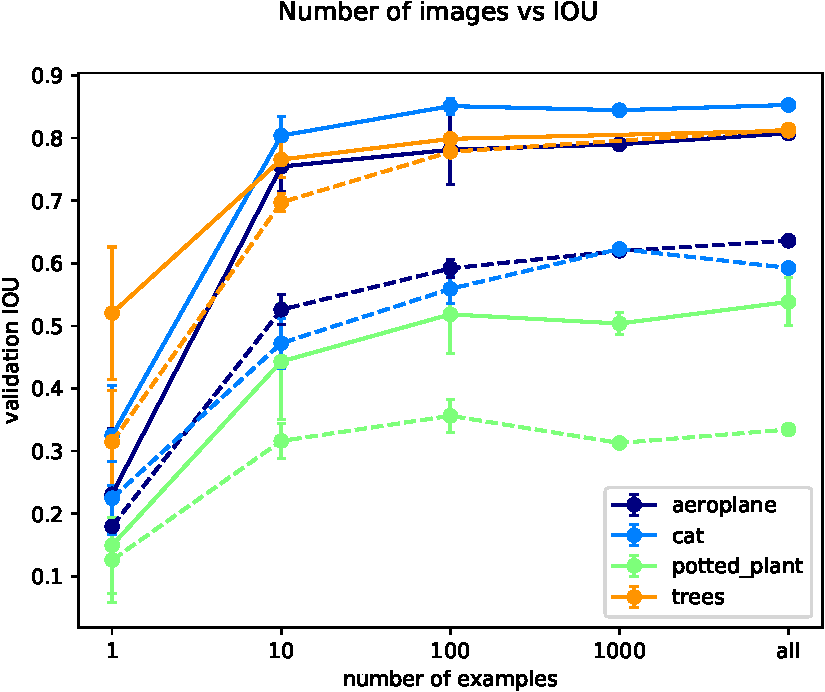
\includegraphics[width=0.9\linewidth]{bootstrap/limit.pdf}
\caption{Validation with a limited number of images, solid line is with the pre-trained model}  
\label{fig:limited}
\end{figure}



\subsection{Model fine-tuning}

We examined the best parameters for fine tuning, finding that allowing a small learning rate on the pre-trained model was advantageous. The effects can be seen in Figure \ref{fig:fine}, where $0.01$ (fraction of the learning rate used for other parts of the model) was advantageous. We used $ 0.1 $ for all other experimentation in this paper. It can be seen that without the lower learning rate, the pre-trained parameters are disturbed leading to lower validation accuracy, and without any fine-tuning the pre-trained parameters are not able to adapt.

Depth of the model is examined, we experiment with truncating the pre-trained model. Results can be seen in Figure \ref{fig:depth}, where the depth of the model had a strong positive effect on the output of the model. Given these results we might consider using a model with even more depth scales. Given the number of convolutions (especially at the lower scales), the ResNet--18 model we have been using has quite a large receptive field, with more depth scales the receptive field would be larger. In \cite{Peng2017} benefit was found in using very large kernels at the lower levels of the model specifically to enlarge the receptive field.

\begin{figure*}[!ht]
\centering
\begin{subfigure}{.5\textwidth}
  \centering
  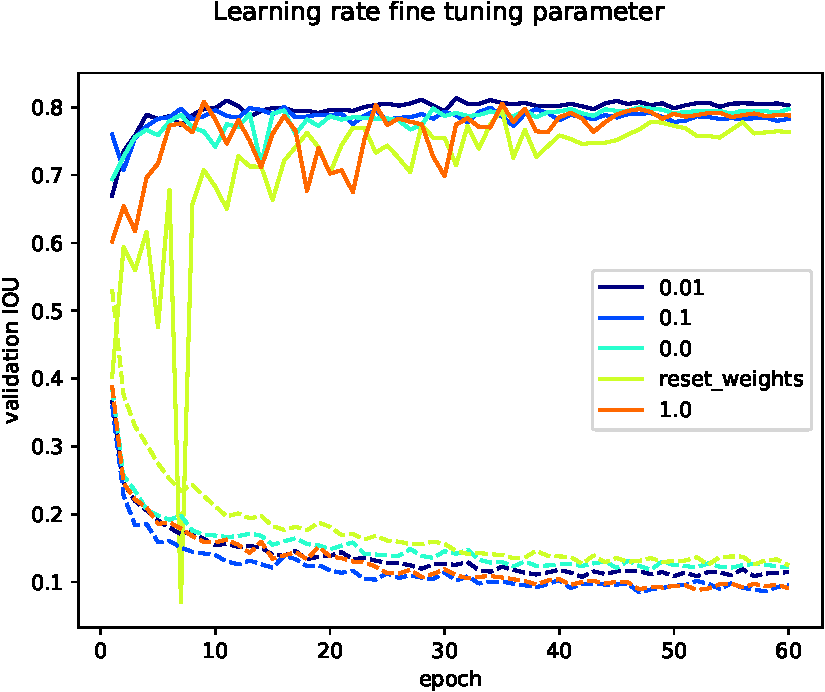
\includegraphics[width=0.9\linewidth]{bootstrap/fine_tuning.pdf}
  \caption{Influence of learning rate modifier for fine tuning}  
  \label{fig:fine}
\end{subfigure}%
\begin{subfigure}{.5\textwidth}
  \centering
  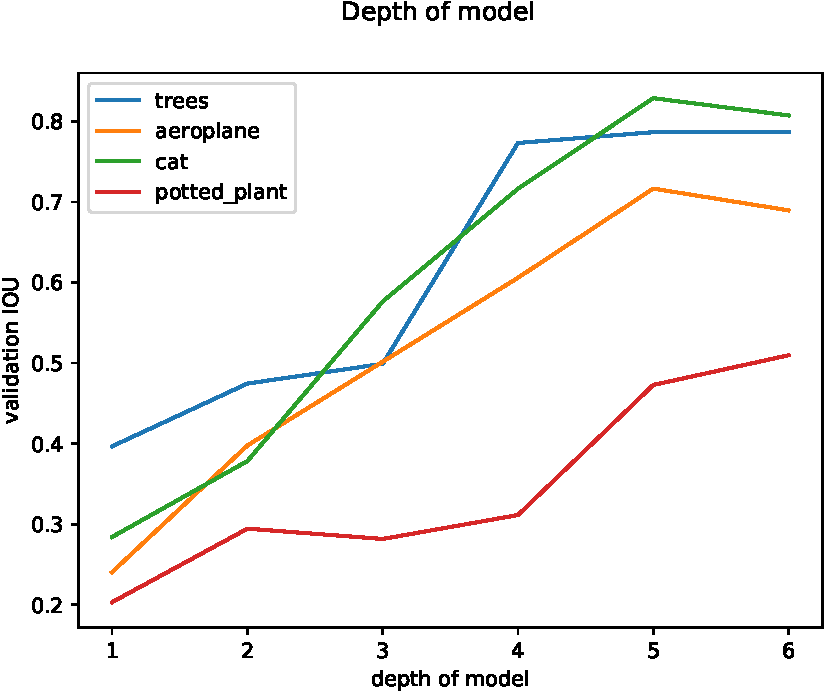
\includegraphics[width=0.9\linewidth]{bootstrap/depth.pdf}
  \caption{Depth of pre-trained model}  
  \label{fig:depth}
\end{subfigure}

\label{fig:training}
\end{figure*}




\subsection {Partial Annotation}


\begin{figure*}[!ht]
\centering
\begin{subfigure}[t]{.3\textwidth}
  \centering
  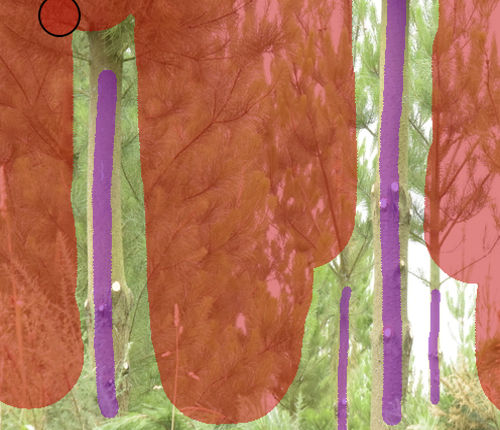
\includegraphics[width=0.6\linewidth]{bootstrap/loose.png}
  \caption{Partial annotation}
  \label{fig:loose_annot}
\end{subfigure}%
\begin{subfigure}[t]{.3\textwidth}
  \centering
  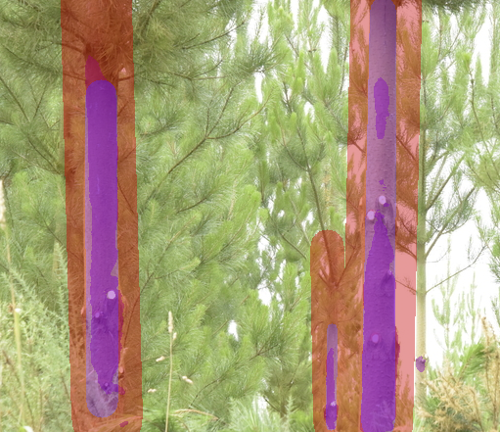
\includegraphics[width=0.6\linewidth]{bootstrap/loose_directed.png}
  \caption{Directed annotation}
  \label{fig:loose_dir}

\end{subfigure}%
\begin{subfigure}[t]{.3\textwidth}
  \centering
  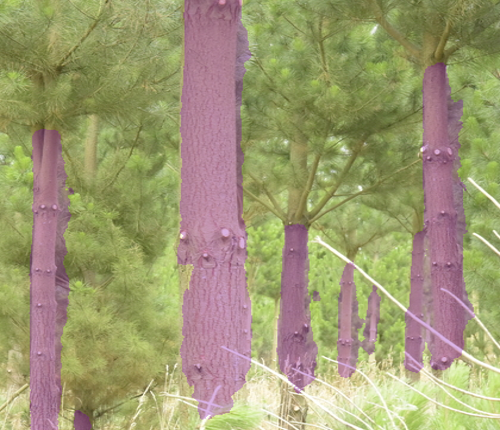
\includegraphics[width=0.6\linewidth]{bootstrap/loose_predictions.png}
  \caption{Predictions from partial annotation showing failure cases}
  \label{fig:loose_pred}
\end{subfigure}
  \caption{Loose annotation methods, red overlay refers to pixels labelled as background where transparent pixels are unlabelled}


\end{figure*}

\begin{figure}
\centering
\begin{subfigure}[t]{.15\textwidth}
  \centering
  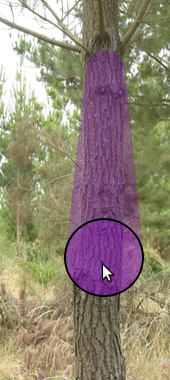
\includegraphics[width=0.7\linewidth]{bootstrap/line_tool.png}
  \caption{Line tool}
\end{subfigure}%
\begin{subfigure}[t]{.15\textwidth}
  \centering
  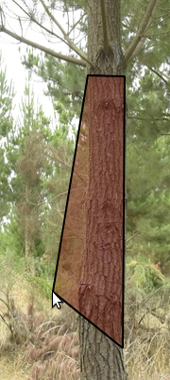
\includegraphics[width=0.7\linewidth]{bootstrap/polygon_tool.png}
  \caption{Polygon tool}
\end{subfigure}%
\begin{subfigure}[t]{.15\textwidth}
  \centering
  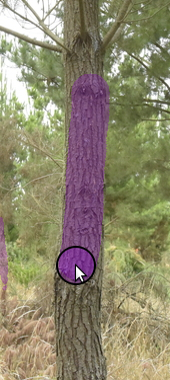
\includegraphics[width=0.7\linewidth]{bootstrap/paint_tool.png}
  \caption{Paint tool}
\end{subfigure}%

  \caption{Label paint tools used in annotation}
  \label{fig:tools}

\end{figure}



An alternative to densely annotating every pixel in an image is to selectively label some pixels while leaving many unlabelled - in the vein of the GrabCut algorithm. We examine this idea for a couple of reasons, firstly annotation all pixels is finicky or ambiguous (such as the small trees in the background), or secondly to optimise time spent on annotation only the most informative pixels (in the vein of active learning).

We firstly looked at partial annotation using paintbrush scribbles on the centre of trees and around the edges of the background. It can be seen that the model trained with partial annotation does not accurately find tree boundaries and has poor precision as a result as can be seen in Figure \ref{fig:loose_pred}. After identifying flaws in that process we compared directed annotation where we trained a model as we went in order to guide the annotation process.

For directed annotation we densely labelled the tree instances where there were mistakes, making sure to more accurately capture the boundaries. We were again annotating only a small number of easier instances where annotation was clear, unlike in the dense annotation case where many small and ambiguous instances are labelled.

Some statistics can be seen in table \ref{tab:loose_exp}, where we can see that both methods of partial annotation are less effective than dense annotation. The second method of directed annotation improves on the precision, but sacrifices recall. We can see that the extra supervision is indeed useful, and we lose useful supervision by not validating the model's correct output as well as fixing it's mistakes.


\begin{table}[!ht]
  \centering
    \caption{Statistics from re-annotation test set}

\noindent\resizebox{0.5\textwidth}{!}{%        
  \begin{tabular}{ l  l  l l l l l }
    Method & Positive pixels & Background pixels & Ignored pixels & Precision & Recall & IOU  \\
    \toprule
    Dense annotation	& 10.4\% & 89.6\% & 0\% & 87.8 & 87.3 & 77.8 \\
    Loose annotation	& 5.2\% & 67.4\% & 27.4\% & 82.3 & 83.3 & 70.7 \\
    Directed annotation & 7.2\% & 54.9\% & 38.0\% & 87.7 & 80.7 & 72.5 \\    
    \bottomrule
  \end{tabular}
}

\label{tab:loose_exp}
\end{table}






\subsection {Annotation interface experiment}



We performed an exercise in re-annotating the validation set using different tools. The results can be seen in table \ref{tab:annotation_exp}, where we used three approaches. The different tools used can be seen above in Figure \ref{fig:tools}.  The first being a duplication of the initial annotation using the line tool (the tool we initially used to label the dataset), the second being a polygon tool (more commonly used and general purpose than the line tool), and lastly we refined images produced by a trained model, fixing mistakes using the paint tool.

The model we used was a model trained on 30 images (densely labelled) from the loose annotation experiment above. We can see the method of refining model predictions is somewhat faster than the other two input methods, but due to the exercise being undertaken by a single user not significantly different ($ p > 0.01 $).

During the annotation we showed an image of the existing validation image and it's annotations side by side to the annotation software, this was necessary to ensure the same task was being performed. The smaller instances in each image were subject to the judgement of the annotator, and other images were extremely crowded or blurry leading to ambiguity in the annotation process. 



We can see from this exercise how tricky , given that two annotations using the same tool and using the other as a reference guide only managed a precision and recall of approximately $ 90\% $. All three methods were similar in this regard, but displayed different bias. The polygon tool for example (as used by the particular annotator) was more precise but less complete (lower recall), indicating that the user tended to cut within boundaries defined by the original labelling. 




\begin{table*}[!ht]
  \centering
    \caption{Statistics from annotating validation set in different ways. Precision, recall and IOU are a comparison with the original validation set. Note figures in brackets are the original statistics of the un-modified predictions from the model}

\noindent\resizebox{\textwidth}{!}{%    
  \begin{tabular}{ l  l  l  l  l  l  l  l }
    Method & Time/image & Edits/image & Pixels/image & Time/edit & Precision & Recall & IOU \\
    \toprule
    Polygon tool	& $79.3 \pm 35.0$  & $12.1 \pm 5.6$ & $52438 \pm 31900$   & $3.9 \pm 1.8$  & $0.94$ & $0.88$   & $0.84$ \\
    Line tool 		& $71  \pm 33.4$   & $12.2 \pm 5.6$ & $54781 \pm 33336$   & $2.1 \pm 1.4$ & $0.92$  & $0.90$  & $0.84$ \\
    Refine from model 	& $57.3 \pm 40.3$  & $10.8 \pm 6.1$ & $6561 \pm 7102$ 	  & $1.7 \pm 1.4$ & $0.92 (0.89)$   & $0.92 (0.85)$ & $0.85 (0.77)$ \\    
    \bottomrule
  \end{tabular}
}

\label{tab:annotation_exp}
\end{table*}


The confounding feature the annotation experiment was the need to look backward and forward between the two images in order to ensure the correct areas were annotated. In images with many instances, this became a difficult task and identifying small differences between the two became much more difficult. In future we may perform a more comprehensive user study, by providing an outline of the desired mask for the user to copy directly. This way the user does not spend any time comparing images and can focus only on the interaction (as a normal user of the annotation tool would).


\subsection{Practical considerations}

The need for more traditional validation for determining hyper--parameters, (for example training rate, model architecture) still need to be determined by validation as soon as enough examples have been obtained to be feasible. We performed some tuning of the hyper--parameters (for example the crop size, data augmentation parameters, learning rate) for the purposes of the experiments in this paper using the person category of the Pascal \gls{VOC} 2012 dataset, despite the fact that the tree dataset is significantly faster to train a similar set of hyper--parameters seems to have been suitable.


A practical consideration of having a process training a \gls{CNN} in the background, is that it uses a lot of (both CPU and GPU) resources. Running the trainer and the annotation tool together caused significant lag in the annotation tool which was not otherwise present and especially noticeable with a large batch size, the tool would lag in sync with each batch processed. The effect was that annotation became somewhat more time consuming. A simple solution to this would be to run processes on different machines with a web interface, for example.


\section{Future work}


In the future we intend to focus on more sophisticated methods of assisted annotation. We have already implemented some preliminary ideas, for example GrabCut with RGB-P such as proposed in \cite{Xu2016a}, utilising the model's predictions as another image channel.  Enhanced SuperPixels is another idea, however we found despite some improvement it suffered from many of the same problems as plain SuperPixels for small instances. 

In initially labelling our tree dataset we used drawing tools to create pixel masks, the problem with with pixel masks is twofold - firstly it is possible (and probable) for a model to make noisy predictions, secondly the pixel masks are not as easy to manipulate than the original primitives. For that reason we are interested in higher level prediction, where the model predicts the same high level primitives as the user first uses for input allowing for the full round trip. For example with our tree data set we draw trees using a line tool, then have the model predict those lines directly.


\section {Conclusion}

We proposed a bootstrapping method for rapid segmentation dataset creation, involving a feedback loop between human and model. The model trained on partial data is used to assist a human annotator, which then verifies the model's predictions and fixes any mistakes. We used this method to create a tree dataset for segmentation of Pinus Radiata trunks (for the purpose of finding trees requiring pruning). We then performed several experiments on this dataset, as well as the Pascal VOC in order to see how we might improve on this basic bootstrapping method. 

Through several experiments we determine that fine-tuning a pre-trained model is an effective way to obtain a workable model with very few input images, at least on our tree dataset. Partial annotation was explored and found to be less effective than a dense annotation. For this reason we think that it is more useful to create tools to assist the user to create a dense annotation, rather than making do with more approximate labelling. Alternatively in future we may focus on methods allowing for a round trip using high level primitives.


\bibliography{library}
